% -*- latex -*-
% FILE: "/home/evmik/jobs/wm/2012_spring_Analog_Electronics_252/final_exam/questions/oscillator.tex"
% LAST MODIFICATION: "Tue, 01 May 2012 14:21:05 -0400 (evmik)"
% (C) 2011 by Eugeniy Mikhailov, <evgmik@gmail.com>
% $Id:$

\question{}
	Consider the relaxation oscillator base on the open collector
	comparator shown below with the following parameters:\\
	$R_1=100$~k$\Omega$, $R_2=100$~k$\Omega$, $R_f=100$~k$\Omega$, and
	$R_{{p.up}}$=1~k$\Omega$.
	\begin{parts}
		\part[2]
		Disregarding $R_{{p.up}}$.
		What is the voltage at non-inverting input when output is
		high?
		\\
		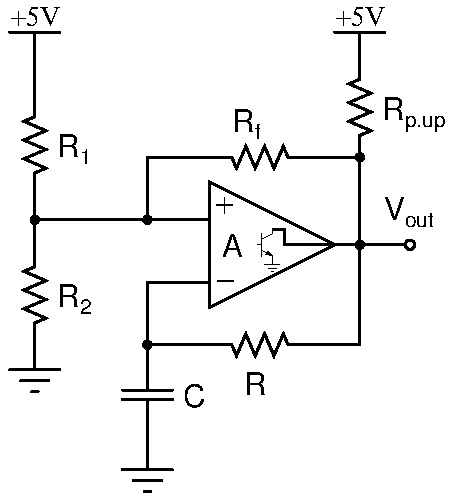
\includegraphics[height=2in]{./schematics/oscillator}
		$V_{+}=$
		\part[2]
		Disregarding $R_{{p.up}}$.
		What is the voltage at non-inverting input when output is
		low?
		\vskip 1.0in
		$V_{+}=$
		\part[4]
		If $R=1$~M$\Omega$, what is the value of the capacitor to
		get period of oscillation T=$1$~mS?
		\vskip 1.0in
		$C=$
		\part[2]
		Can we completely get rid of $R_{p.up}$? Why?
		\vskip 1.0in
		\bonuspart[5]
		When we built a blinker, we learn that hooking an LED
		directly to the output is bad idea die to large output
		impedance in comparison to the small input impedance of the
		LED. What is the output impedance of this circuit? {\bf
		Show} your reasons.
		\vskip 1.0in
		$Z_{out}=$
	\end{parts}
	\pagebreak

